\chapter{Généralités sur les fonctions}

\section{Définitions et notations}

\subsection{Définition}

\begin{ex}
	\nline
	\begin{wrapstuff}[r]
		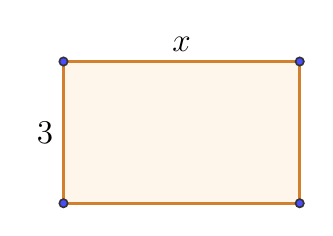
\begin{tikzpicture}[thick, scale=0.6]
			\coordinate (A) at (0,0);
			\coordinate (B) at (5,0);
			\coordinate (C) at (5,3);
			\coordinate (D) at (0,3);
			\filldraw[draw=brown!70!orange, fill=brown!12!orange!8, line width=1pt] (A) -- (B) -- (C) -- (D) -- cycle;
			\node[above, font=\large] at (2.5,3) {$x$};
			\node[left, font=\large] at (0,1.5) {$3$};
			\foreach \point in {A, B, C, D} { \filldraw[fill=blue!70!white, draw=black!80, line width=0.6pt] (\point) circle (2.5pt); }
		\end{tikzpicture}
	\end{wrapstuff}

	On considère la fonction $f$ qui donne l'aire d'un rectangle de dimensions $3$ et $x$.

	Une \textbf{expression littérale} de $f$ est donc :
	\[
		f(x)=3x
	\]

	\phantom{x}
\end{ex}

\begin{defin}
	Une fonction $f$ associe à tout nombre réel $x$ un unique nombre réel, noté $f(x)$.

	On note également :
	\[
		x\mapsto f(x)\quad\text{ou}\quad y=f(x)
	\]
\end{defin}

\begin{ex}
	\nline
	\begin{wrapstuff}
		\begin{tikzpicture}[>=Stealth, thick, scale=1.1]
			\draw[line width=3pt, gray!40, line cap=round] (-3,-0.8) -- (3,-0.8);
			\foreach \x in {-2.5,-2,-1.5,1.5,2,2.5} { \draw[gray!60, thin] (\x, -0.8) circle (2pt); }
			\node[draw=gray!40, fill=gray!5, rounded corners=2pt, font=\small, text=gray!80!black] at (-3,-0.5) {$9.1$};
			\node[draw=gray!40, fill=gray!5, rounded corners=2pt, font=\small, text=gray!80!black] at (-2.2,-0.5) {$-5$};
			\node[draw=gray!40, fill=gray!5, rounded corners=2pt, font=\small, text=gray!80!black] at (-1.4,-0.5) {$12$};
			\node[draw=gray!40, fill=gray!5, rounded corners=2pt, font=\small, text=gray!80!black] at (1.5,-0.5) {$7.3$};
			\node[draw=gray!40, fill=gray!5, rounded corners=2pt, font=\small, text=gray!80!black] at (2.2,-0.5) {$2$};
			\node[draw=gray!40, fill=gray!5, rounded corners=2pt, font=\small, text=gray!80!black] at (3,-0.5) {$-9.2$};
			\filldraw[draw=blue!70!black, fill=blue!10, rounded corners=12pt, line width=1.5pt] (-1.5,-1) rectangle (1.5,1.2);
			\filldraw[fill=blue!60!black] (-1,1.2) -- (-0.8,1.4) -- (0.8,1.4) -- (1,1.2) -- cycle;
			\node[text=blue!90!black, font=\sffamily\bfseries] at (0,0.6) {Fonction $f$};
			\node[draw=orange!70, fill=orange!5, rounded corners=4pt, inner sep=5pt, font=\sffamily\large\bfseries, text=orange!90!black] at (0,-0.1) {$2x + 1$};
			\node[draw=gray!60, fill=white, circle, inner sep=4pt, font=\large\bfseries] (In) at (-3,0.3) {$x$};
			\draw[->, line width=1.5pt, green!60!black] (-2.4,0.3) -- (-1.6,0.3);
			\node[above, font=\sffamily\small\bfseries, text=green!60!black] at (-2.1, 0.4) {Entrée};
			\node[draw=gray!60, fill=white, circle, inner sep=1pt, font=\large\bfseries] (Out) at (3,0.3) {$f(x)$};
			\draw[->, line width=1.5pt, red!70!black] (1.6,0.3) -- (2.4,0.3);
			\node[above, font=\sffamily\small\bfseries, text=red!70!black] at (2.1, 0.4) {Sortie};
		\end{tikzpicture}
	\end{wrapstuff}

	Voici des exemples de fonctions :

	\begin{itemize}
		\item $f(x)=2x+1$
		\item $g: x\mapsto\dfrac{x}{\sqrt{x}}$
		\item $h(x)=1+x+\dfrac{x^2}{2}+\frac{x^3}{6}$
		\item $i(x)=\dfrac{3x+1}{x^2}$
	\end{itemize}
\end{ex}

\subsection{Image et antécédent}

\begin{ex}
	Dire que $~f(2)=5~$ signifie que $~2\mapsto 5$

	On dit que :
	\begin{itemize}
		\item l'\textbf{image} de $2$ par la fonction $f$ est $5$.
		\item un \textbf{antécédent} de $5$ par $f$ est $2$.
	\end{itemize}
\end{ex}

\begin{rem}
	\nline
	\begin{itemize}
		\item Un nombre possède une \textbf{unique image}.
		\item Cependant, un nombre peut posséder plusieurs antécédents.
	\end{itemize}
\end{rem}

\begin{methode}[Déterminer l'image d'une fonction par calcul]
	\nline
	\begin{wrapstuff}[r]
		\begin{tikzpicture}[>=Stealth, thick, scale=1.1]
			\draw[line width=3pt, gray!40, line cap=round] (-3,-0.8) -- (3,-0.8);
			\foreach \x in {-2.5,-2,-1.5,1.5,2,2.5} { \draw[gray!60, thin] (\x, -0.8) circle (2pt); }
			\node[draw=gray!40, fill=gray!5, rounded corners=2pt, font=\small, text=gray!80!black] at (-2.2,-0.5) {$6$};
			\node[draw=gray!40, fill=gray!5, rounded corners=2pt, font=\small, text=gray!80!black] at (2.2,-0.5) {$34$};
			\filldraw[draw=blue!70!black, fill=blue!10, rounded corners=12pt, line width=1.5pt] (-1.5,-1) rectangle (1.5,1.2);
			\filldraw[fill=blue!60!black] (-1,1.2) -- (-0.8,1.4) -- (0.8,1.4) -- (1,1.2) -- cycle;
			\node[text=blue!90!black, font=\sffamily\bfseries] at (0,0.6) {Fonction $g$};
			\node[draw=orange!70, fill=orange!5, rounded corners=4pt, inner sep=5pt, font=\sffamily\large\bfseries, text=orange!90!black] at (0,-0.1) {$x^2-2$};
			\node[draw=gray!60, fill=white, circle, inner sep=4pt, font=\large\bfseries] (In) at (-3,0.3) {$x$};
			\draw[->, line width=1.5pt, green!60!black] (-2.4,0.3) -- (-1.6,0.3);
			\node[above, font=\sffamily\small\bfseries, text=green!60!black] at (-2.1, 0.4) {Entrée};
			\node[draw=gray!60, fill=white, circle, inner sep=1pt, font=\large\bfseries] (Out) at (3,0.3) {$g(x)$};
			\draw[->, line width=1.5pt, red!70!black] (1.6,0.3) -- (2.4,0.3);
			\node[above, font=\sffamily\small\bfseries, text=red!70!black] at (2.1, 0.4) {Sortie};
		\end{tikzpicture}
	\end{wrapstuff}
	Soit la fonction $g$ définie par $g(x)=x^{2}-2$.

	Calculons l'image de $6$ par la fonction $g$.

	\cmath{\begin{aligned}g(6)&=6^{2}-2\\\quad&=36-2\quad=34\end{aligned}}

	L'image de $6$ par la fonction $g$ est $34$.
\end{methode}

\newpage

\begin{methode}[Déterminer un antécédent par calcul]
	\nline
	\begin{wrapstuff}[r]
		\begin{tikzpicture}[>=Stealth, thick, scale=1.1]
			\draw[line width=3pt, gray!40, line cap=round] (-3,-0.8) -- (3,-0.8);
			\foreach \x in {-2.5,-2,-1.5,1.5,2,2.5} { \draw[gray!60, thin] (\x, -0.8) circle (2pt); }
			\node[draw=gray!40, fill=gray!5, rounded corners=2pt, font=\small, text=gray!80!black] at (-2.2,-0.5) {$-1$};
			\node[draw=gray!40, fill=gray!5, rounded corners=2pt, font=\small, text=gray!80!black] at (2.2,-0.5) {$-5$};
			\filldraw[draw=blue!70!black, fill=blue!10, rounded corners=12pt, line width=1.5pt] (-1.5,-1) rectangle (1.5,1.2);
			\filldraw[fill=blue!60!black] (-1,1.2) -- (-0.8,1.4) -- (0.8,1.4) -- (1,1.2) -- cycle;
			\node[text=blue!90!black, font=\sffamily\bfseries] at (0,0.6) {Fonction $f$};
			\node[draw=orange!70, fill=orange!5, rounded corners=4pt, inner sep=5pt, font=\sffamily\large\bfseries, text=orange!90!black] at (0,-0.1) {$2x-3$};
			\node[draw=gray!60, fill=white, circle, inner sep=4pt, font=\large\bfseries] (In) at (-3,0.3) {$x$};
			\draw[->, line width=1.5pt, green!60!black] (-2.4,0.3) -- (-1.6,0.3);
			\node[above, font=\sffamily\small\bfseries, text=green!60!black] at (-2.1, 0.4) {Entrée};
			\node[draw=gray!60, fill=white, circle, inner sep=1pt, font=\large\bfseries] (Out) at (3,0.3) {$f(x)$};
			\draw[->, line width=1.5pt, red!70!black] (1.6,0.3) -- (2.4,0.3);
			\node[above, font=\sffamily\small\bfseries, text=red!70!black] at (2.1, 0.4) {Sortie};
		\end{tikzpicture}
	\end{wrapstuff}
	Soit la fonction $f$ définie par $f(x)=2x-3$.

	Déterminons un antécédent de $\pa{-5}$ par la fonction $f$.

	On peut donc écrire :
	\[
		f(x)=-5\quad\iff\quad 2x-3=-5
	\]

	On résout ainsi l'équation :

	\cmath{
		\begin{array}{rrl}
			     & f(x) = & -5                            \\
			\iff & 2x-3 = & (-5)                          \\
			\iff & 2x =   & -5+3                          \\
			\iff & 2x =   & (-2)\qquad\iff\quad x=\pa{-1}
		\end{array}
	}

	L'antécédent de $(-5)$ par $f$ est donc $(-1)$.
\end{methode}

\subsection{Ensemble de définition}

\begin{df}
	L'\textbf{ensemble de définition} d'une fonction $f$, noté $\mathcal{D}$ ou $\mathcal{D}_f$, est l'ensemble de tous les nombres réels $x$ pour lesquels il est possible de calculer l'image $f(x)$.
\end{df}

\begin{ex}
	\nline
	\begin{itemize}
		\item Pour la fonction $f(x)=2x+1$, on peut calculer l'image de n'importe quel nombre réel.

		      Son ensemble de définition est $\mathcal{D}_f=\R$.
		\item Pour la fonction $g(x)=\dfrac{1}{x}$, on ne peut pas diviser par $0$. La valeur $0$ est interdite.

		      L'ensemble de définition est $\mathcal{D}_f=\R \setminus \{0\}$.
	\end{itemize}
\end{ex}

\section{Représentation graphique}

\begin{methode}{Représenter graphiquement une fonction}
	Soit la fonction $f$ définie sur $\intff{0}{5}$ par :
	\[
		f(x)=5x-x^{2}
	\]

	Pour représenter la fonction $f$, il faut calculer quelques images de nombres :

	\begin{multicols}{3}
		\begin{itemize}
			\item $f(0)=5\times 0-0^2=0$
			\item $f(1)=5\times 1-1^2=4$
			\item $f(2)=5\times 2-2^2=6$
			\item $f(3)=5\times 3-3^2=6$
			\item $f(4)=5\times 4-4^2=4$
			\item $\ldots$
		\end{itemize}
	\end{multicols}

	On consigne nos résultats dans un tableau de valeurs :
	\[
		\def\arraystretch{1.8}
		\begin{array}{|>{\ccg}c|C{1cm}|C{1cm}|C{1cm}|C{1cm}|C{1cm}|C{1cm}|C{1cm}|C{1cm}|C{1cm}|C{1cm}|}\hline
			x    & $0$ & $1$ & $1,5$  & $2$ & $2,5$  & $3$ & $3,5$  & $4$ & $4,5$  & $5$ \\ \hline
			f(x) & $0$ & $4$ & $5,25$ & $6$ & $6,25$ & $6$ & $5,25$ & $4$ & $2,25$ & $0$ \\ \hline
		\end{array}
	\]

	On représente les données du tableau de valeurs dans un repère tel que :
	\begin{itemize}
		\item Les valeurs de $x$ se trouvent \textbf{en abscisse}
		\item Les valeurs de $f(x)$ correspondantes se trouvent \textbf{en ordonnée}.
	\end{itemize}

	\begin{center}
		\hfill
		\begin{tikzpicture}[>=Stealth, scale=0.7, every node/.style={transform shape}]
			\draw[gray!40, thin] (-0.8,-1.5) grid (5.5,6.8);
			\draw[->, line width=1.1pt] (-0.8,0) -- (5.6,0);
			\draw[->, line width=1.1pt] (0,-1.5) -- (0,6.9);
			\node[below left] at (0,0) {$0$};
			\foreach \x in {1,2,3,4,5} { \draw[line width=0.8pt] (\x,2pt) -- (\x,-2pt) node[below, yshift=-2pt] {$\x$}; }
			\foreach \y in {-1,1,2,3,4,5,6} { \draw[line width=0.8pt] (2pt,\y) -- (-2pt,\y) node[left, xshift=-2pt] {$\y$}; }
			\tikzset{pt/.style={circle, fill=black, draw=black, inner sep=0pt, minimum size=5pt}}
			\node[pt] at (0,0) {};
			\node[pt] at (1,4) {};
			\node[pt] at (1.5,5.25) {};
			\node[pt] at (2,6) {};
			\node[pt] at (2.5,6.25) {};
			\node[above right,fill=white,yshift=1pt] at (3,6) {$\coordl{3}{6}$};
			\node[pt] at (3,6) {};
			\node[pt] at (3.5,5.25) {};
			\node[above right,fill=white,yshift=1pt] at (4,4) {$\coordl{4}{4}$};
			\node[pt] at (4,4) {};
			\node[pt] at (4.5,2.25) {};
			\node[pt] at (5,0) {};
		\end{tikzpicture}
		\hfill$\rarr$\hfill
		\begin{tikzpicture}[>=Stealth, scale=0.7, every node/.style={transform shape}]
			\draw[gray!40, thin] (-0.8,-1.5) grid (5.5,6.8);
			\draw[->, line width=1.1pt] (-0.8,0) -- (5.6,0);
			\draw[->, line width=1.1pt] (0,-1.5) -- (0,6.9);
			\node[below left] at (0,0) {$0$};
			\foreach \x in {1,2,3,4,5} { \draw[line width=0.8pt] (\x,2pt) -- (\x,-2pt) node[below, yshift=-2pt] {$\x$}; }
			\foreach \y in {-1,1,2,3,4,5,6} { \draw[line width=0.8pt] (2pt,\y) -- (-2pt,\y) node[left, xshift=-2pt] {$\y$}; }
			\draw[line width=2pt, green!50!black, samples=100, domain=0:5] plot (\x, {-(\x-2.5)*(\x-2.5)+6.25});
			\tikzset{pt/.style={circle, fill=black, draw=black, inner sep=0pt, minimum size=5pt}}
			\node[pt] at (0,0) {};
			\node[pt] at (1,4) {};
			\node[pt] at (1.5,5.25) {};
			\node[pt] at (2,6) {};
			\node[pt] at (2.5,6.25) {};
			\node[pt] at (3,6) {};
			\node[pt] at (3.5,5.25) {};
			\node[pt] at (4,4) {};
			\node[pt] at (4.5,2.25) {};
			\node[pt] at (5,0) {};
		\end{tikzpicture}
		\hfill~
	\end{center}
\end{methode}

\begin{rem}
	\nline
	\begin{itemize}
		\item Les \textbf{images} $f(x)$ se lisent sur l'\textbf{axe des ordonnées} $\pa{y}$.
		\item La courbe représentative de $f$ définie par $~f(x)=5x-x^{2}~$ peut se noter : $~y=5x-x^{2}$
		\item De façon générale, l'équation d'une courbe se note $~y=f(x)$
	\end{itemize}
\end{rem}

\section{Résolution graphique d'équations et d'inéquations}

\begin{methode}[Résoudre graphiquement une équation]
	\nline
	\begin{wrapstuff}[r]
		\begin{tikzpicture}[>=Stealth,scale=0.8]
			\draw[gray!40, dashed, line width=0.6pt] (-0.5,-0.5) grid (5.5,6.5);
			\draw[->, line width=1pt] (-0.5,0) -- (5.6,0);
			\draw[->, line width=1pt] (0,-0.5) -- (0,6.6);
			\node[below left] at (0,0) {$0$};
			\foreach \x in {2,3,5} { \node[below, yshift=-2pt] at (\x,0) {$\x$}; }
			\node[below, red, font=\bfseries, yshift=-2pt] at (1,0) {$1$};
			\node[below, red, font=\bfseries, yshift=-2pt] at (4,0) {$4$};
			\foreach \y in {1,2,3,5,6} { \node[left, xshift=-2pt] at (0,\y) {$\y$}; }
			\node[left, green!60!black, font=\bfseries, xshift=-2pt] at (0,4) {$4$};
			\draw[line width=2pt, black!80, samples=100, domain=0:5] plot (\x, {-\x*\x + 5*\x});
			\tikzset{fleche_verte/.style={->, >=Stealth, line width=1.5pt, green!60!black}}
			\draw[fleche_verte] (0,4) -- (4,4);
			\draw[fleche_verte] (1,4) -- (1,0.05);
			\draw[fleche_verte] (4,4) -- (4,0.05);
		\end{tikzpicture}
	\end{wrapstuff}
	On a représenté la courbe de $f$ définie par :
	\[
		f(x)=5x-x^{2}
	\]

	Résolvons \textbf{graphiquement} l'équation :
	\[
		5x-x^{2}=4\iff f(x)=4
	\]

	Ce qui revient à trouver des antécédents de $4$ par la fonction $f$.

	\begin{itemize}
		\item On "part" de l'ordonnée $4$
		\item On "rejoint" la courbe
		\item On lit les solutions sur l'axe des abscisses
	\end{itemize}

	On a :
	\[
		f(x)=4~\iff~\begin{cases}x=1\\x=4\end{cases}
	\]

	On peut noter :
	\[
		f(x)=4\iff S=\left\{ 1;4 \right\}
	\]
\end{methode}

\begin{rem}
	\nline
	\begin{itemize}
		\item Par \textbf{lecture graphique}, les solutions obtenues sont \textbf{approchées}.
		\item L'équation $f(x)=7$, ne semble pas avoir de solution car la courbe représentée ne possède pas de point d'ordonnée $7$.
		\item \textbf{Graphiquement}, on ne peut pas être certain que les solutions qui apparaissent sont les seules.

		      Il pourrait y en avoir d'autres au-delà des limites de la représentation graphique tracée.
	\end{itemize}
\end{rem}

\newpage

\begin{methode}[Résoudre graphiquement une inéquation]
	\nline
	\begin{wrapstuff}[r]
		\begin{tikzpicture}[>=Stealth, scale=0.8]
			\draw[gray!40, dashed, line width=0.6pt] (-0.5,-0.5) grid (5.5,6.5);
			\draw[->, line width=1pt] (-0.5,0) -- (5.6,0);
			\draw[->, line width=1pt] (0,-0.5) -- (0,6.6);
			\node[below left] at (0,0) {$0$};
			\foreach \x in {2,3,5} { \node[below, yshift=-2pt] at (\x,0) {$\x$}; }
			\foreach \y in {1,2,3,5,6} { \node[left, xshift=-2pt] at (0,\y) {$\y$}; }
			\node[below, red, font=\bfseries\large, yshift=-4pt] at (1,0) {$1$};
			\node[below, red, font=\bfseries\large, yshift=-4pt] at (4,0) {$4$};
			\node[left, green!60!black, font=\bfseries\large, xshift=-2pt] at (0,4) {$4$};
			\draw[red, line width=3.5pt] (1,0) -- (4,0);
			\draw[red, line width=1.8pt] (0.85, 0.25) -- (1, 0.25) -- (1, -0.25) -- (0.85, -0.25);
			\draw[red, line width=1.8pt] (4.15, 0.25) -- (4, 0.25) -- (4, -0.25) -- (4.15, -0.25);
			\draw[line width=1pt, black!80, samples=100, domain=-0:5] plot (\x, {-\x*\x + 5*\x});
			\draw[line width=3.5pt, red, samples=50, domain=1:4] plot (\x, {-\x*\x + 5*\x});
			\tikzset{flecheverte/.style={->, >=Stealth, line width=1.5pt, green!60!black}}
			\draw[flecheverte] (0,4) -- (4,4);
			\draw[flecheverte] (1,4) -- (1,0.27); % s'arrête juste au-dessus du crochet
			\draw[flecheverte] (4,4) -- (4,0.27); % s'arrête juste au-dessus du crochet
		\end{tikzpicture}
	\end{wrapstuff}
	Dans la méthode précédente, on a représenté la fonction $f$ définie par :
	\[
		f(x)=5x-x^{2}
	\]

	Résolvons \textbf{graphiquement} l'inéquation :
	\[
		5x-x^{2}>4\iff f(x) > 4
	\]

	L'inéquation $~\pa{5x-x^{2}}>4~$ peut s'écrire $~f(x)>4$.

	Ce qui revient à déterminer les abscisses des points de la courbe dont l'\textbf{ordonnée est strictement supérieure} à $4$.

	On lit les solutions sur l'axe des abscisses et on peut noter :
	\[
		f(x)>4\iff S=\intoo{1}{4}
	\]
\end{methode}

\section{Variations d'une fonction}

\subsection{Taux de variation}

\begin{defin}
	Le \textbf{taux de variation} de la fonction $f$ entre $a$ et $b$ est le nombre :
	\[
		{\text{Taux de variation}=\dfrac{f(b)-f(a)}{b-a}}
	\]

	\begin{center}
		\begin{tikzpicture}[>=Stealth, scale=0.5]
			\draw[->, line width=1.1pt] (-1,0) -- (6.8,0);
			\draw[->, line width=1.1pt] (0,-1) -- (0,7);
			\draw[line width=1pt, green!50!black, samples=150, domain=-1:6.3] plot (\x, {-0.1*\x*\x*\x + 0.5*\x*\x + 0.8*\x + 1.5});
			\coordinate (A) at (1, 2.7);
			\draw[dashed, line width=0.9pt, black!40] (A) -- (1, 0);
			\draw[dashed, line width=0.9pt, black!40] (A) -- (0, 2.7);
			\coordinate (B) at (4, 6.3);
			\draw[dashed, line width=0.9pt, black!40] (B) -- (4, 0);
			\draw[dashed, line width=0.9pt, black!40] (B) -- (0, 6.3);
			\tikzset{pt_axe/.style={circle, fill=black, inner sep=0pt, minimum size=3.5pt}}
			\tikzset{pt_inter/.style={circle, fill=black, line width=0.8pt, inner sep=0pt, minimum size=3.5pt}}
			\draw[line width=1pt, dotted, black!75, domain=-1:4.8] plot (\x, {1.2*\x + 1.5});
			\node[pt_axe] at (0,2.7) {};
			\node[left, font=\bfseries] at (0,2.7) {$f(a)$};
			\node[pt_axe] at (0,6.3) {};
			\node[left, font=\bfseries] at (0,6.3) {$f(b)$};
			\node[pt_axe] at (1,0) {};
			\node[below, font=\bfseries, yshift=-3pt] at (1,0) {$a$};
			\node[pt_inter] at (A) {};
			\node[pt_axe] at (4,0) {};
			\node[below, font=\bfseries, yshift=-3pt] at (4,0) {$b$};
			\node[pt_inter] at (B) {};
		\end{tikzpicture}
	\end{center}
\end{defin}

\begin{prop}
	Le taux de variation de $f$ entre $a$ et $b$ est la pente de la droite passant par les points d'abscisses $a$ et $b$ de la courbe représentative de $f$.
	\[
		\text{coef.dir}=\text{pente}=\dfrac{\text{Montée}}{\text{Avance}}=\dfrac{\Delta y}{\Delta x}=\dfrac{f(b)-f(a)}{b-a}
	\]

	\begin{center}
		\begin{tikzpicture}[>=Stealth, scale=0.7]
			\draw[->, line width=1.1pt] (-1,0) -- (6.8,0);
			\draw[->, line width=1.1pt] (0,-1) -- (0,7);
			\draw[line width=1pt, green!50!black, samples=150, domain=-1:6.3] plot (\x, {-0.1*\x*\x*\x + 0.5*\x*\x + 0.8*\x + 1.5});
			\coordinate (A) at (1, 2.7);
			\draw[dashed, line width=0.9pt, black!40] (A) -- (1, 0);
			\draw[dashed, line width=0.9pt, black!40] (A) -- (0, 2.7);
			\coordinate (B) at (4, 6.3);
			\draw[dashed, line width=0.9pt, black!40] (B) -- (4, 0);
			\draw[dashed, line width=0.9pt, black!40] (B) -- (0, 6.3);
			\tikzset{pt_axe/.style={circle, fill=black, inner sep=0pt, minimum size=3.5pt}}
			\tikzset{pt_inter/.style={circle, fill=black, line width=-1.8pt, inner sep=0pt, minimum size=3.5pt}}
			\draw[line width=1pt, dotted, black!75, domain=-1:4.8] plot (\x, {1.2*\x + 1.5});
			\node[pt_axe] at (0,2.7) {};
			\node[left, font=\bfseries] at (0,2.7) {$f(a)$};
			\node[pt_axe] at (0,6.3) {};
			\node[left, font=\bfseries] at (0,6.3) {$f(b)$};
			\node[pt_axe] at (1,0) {};
			\node[below, font=\bfseries, yshift=-3pt] at (1,0) {$a$};
			\node[pt_inter] at (A) {};
			\node[pt_axe] at (4,0) {};
			\node[below, font=\bfseries, yshift=-3pt] at (4,0) {$b$};
			\node[pt_inter] at (B) {};
			\draw[->, red, line width=1.2pt] (1, 2.7) -- (4, 2.7) node[midway, below, font=\bfseries] {$\Delta x$};
			\draw[->, red, line width=1.2pt] (4, 2.7) -- (4, 6.3) node[midway, right, font=\bfseries, xshift=-2pt] {$\Delta y$};
		\end{tikzpicture}
	\end{center}
\end{prop}

\newpage

\begin{methode}[Déterminer un taux de variation d'une fonction]
	\nline
	\begin{wrapstuff}
		\begin{tikzpicture}[>=Stealth, xscale=1, font=\small, yscale=0.2]
			\draw[->, line width=1.1pt] (-1,0) -- (3.5,0);
			\draw[->, line width=1.1pt] (0,-2) -- (0,21);
			\draw[line width=1.3pt, green!50!black, samples=150, domain=-0.5:3.2] plot (\x, {2*\x*\x + 1});
			\coordinate (A) at (1, 3);
			\draw[dashed, line width=0.9pt, black!40] (A) -- (1, 0);
			\draw[dashed, line width=0.9pt, black!40] (A) -- (0, 3);
			\coordinate (B) at (3, 19);
			\draw[dashed, line width=0.9pt, black!40] (B) -- (3, 0);
			\draw[dashed, line width=0.9pt, black!40] (B) -- (0, 19);
			\tikzset{pt_axe/.style={circle, fill=black, inner sep=0pt, minimum size=4pt}}
			\tikzset{pt_inter/.style={circle, fill=black, inner sep=0pt, minimum size=4pt}}
			\draw[line width=1pt, dotted, black!75, domain=0.4:3.2] plot (\x, {8*\x - 5});
			\draw[->, red, line width=1.2pt] (1, 3) -- (3, 3) node[midway, below, font=\bfseries] {$2$};
			\draw[->, red, line width=1.2pt] (3, 3) -- (3, 19) node[midway, right, font=\bfseries, xshift=-2pt] {$16$};
			\node[pt_axe] at (0,3) {};
			\node[left, font=\bfseries] at (0,3) {$f(1)=3$};
			\node[pt_axe] at (0,19) {};
			\node[left, font=\bfseries] at (0,19) {$f(3)=19$};
			\node[pt_axe] at (1,0) {};
			\node[below, font=\bfseries, yshift=-3pt] at (1,0) {$1$};
			\node[pt_inter] at (A) {};
			\node[pt_axe] at (3,0) {};
			\node[below, font=\bfseries, yshift=-3pt] at (3,0) {$3$};
			\node[pt_inter] at (B) {};
		\end{tikzpicture}
	\end{wrapstuff}
	Soit $f$ la fonction définie sur $\R$ par $\quad f(x)=2x^{2}+1$

	Déterminons le \textbf{taux de variation} entre $1$ et $3$.
	\[
		\def\arraystretch{2.5}
		\begin{array}{rcl}
			\text{Taux de variation} & = & \dfrac{f(3)-f(1)}{3-1}                                 \\
			                         & = & \dfrac{\pa{2 \times 3^{2}+1}-\pa{2\times 1^{2}+1 }}{2} \\
			                         & = & \dfrac{19-3}{2}\quad =\dfrac{16}{2}\quad=8
		\end{array}
	\]

	La pente de la droite passant par les points d'abscisses $1$ et $3$ est égale à $8$.
\end{methode}

\begin{prop}
	Soit $a$ et $b$, deux nombres d'un intervalle $I$ tel que $a < b$.

	Si le taux de variation d'une fonction $f$ entre \textbf{tous} les couples $a$ et $b$ de $I$ est ... :

	\begin{itemize}
		\item \textbf{...positif,}, alors $f$ est \textbf{strictement croissante} sur $I$.
		\item \textbf{...négatif}, alors $f$ est \textbf{strictement décroissante} sur $I$.
		\item \textbf{...nul}, alors $f$ est \textbf{constante} sur I.
	\end{itemize}
\end{prop}

\begin{methode}[Étudier les variations d'une fonction à l'aide du taux de variation]
	Soit $f$ la fonction définie sur $\mathbb{R}$ par :
	\[
		f(x)=5x-3
	\]

	Démontrons que $f$ est \textbf{strictement croissante} sur $\mathbb{R}$.

	On considère deux nombres quelconques $a$ et $b$.

	Le taux de variation de $f$ entre $a$ et $b$ est égal à :
	\[
		\def\arraystretch{2.5}
		\begin{array}{rcl}
			\dfrac{f(b)-f(a)}{b-a} & = & \dfrac{(5b-3)-(5a-3)}{b-a}                             \\
			                       & = & \dfrac{5b-5a}{b-a}\qquad = \dfrac{5(b-a)}{b-a}\quad =5
		\end{array}
	\]

	Or, $~5>0~$ donc $~\dfrac{f(b)-f(a)}{b-a}>0~$ et donc $f$ est \textbf{strictement croissante} sur $\mathbb{R}$.
\end{methode}

\subsection{Tableau de variations}
Pour résumer les comportements d'une fonction (croissante, décroissante ou constante), on regroupe ces informations dans un \textbf{tableau de variations}.

\begin{ex}
	Reprenons la fonction $f$ définie sur l'intervalle $\intff{0}{5}$ dont la courbe a été étudiée précédemment.

	Son tableau de variations est le suivant :
	\begin{center}
		\begin{tikzpicture}
			\tikzset{arrow style/.style={line width=1.3pt, ->, >=Triangle}}
			\tkzTabInit[lgt=1.5, espcl=2]{$x$ / 0.75 , $f$ / 1.5}{$0$, $2{,}5$, $5$}
			\tkzTabVar{-/ $0$ , +/ $6{,}25$ , -/ $0$}
		\end{tikzpicture}
	\end{center}
\end{ex}

\begin{ex}
	Soit $f$ la fonction définie sur l'intervalle $\intff{-2}{2}$ par :
	\[
		f(x) = x^3 - 3x + 1
	\]

	Sa représentation graphique $\mathcal{C}_f$ dans un repère orthogonal est la suivante :

	\begin{center}
		\begin{tikzpicture}[>=Stealth, x=20mm]
			\clip (-2.25,-1.5) rectangle (2.4,3.75);
			\draw[gray!40, thin] (-2.5,-2.5) grid (2.3,3.5);
			\draw[->, line width=1pt] (-2.5,0) -- (2.3,0) node[above] {$x$};
			\draw[->, line width=1pt] (0,-2.5) -- (0,3.6) node[right] {$y$};
			\node[below left] at (0,0) {$0$};
			\foreach \x in {-2,-1,1,2} { \draw (\x,2pt) -- (\x,-2pt) node[below] {$\x$}; }
			\foreach \y in {-2,-1,1,2,3} { \draw (2pt,\y) -- (-2pt,\y) node[left] {$\y$}; }
			\draw[dashed, rouge, thick] (-1,0) -- (-1,3) -- (0,3);
			\draw[dashed, rouge, thick] (1,0) -- (1,-1) -- (0,-1);
			\node[right, vert, fill=white] at (1.5,2) {$\mathcal{C}_f$};
			\draw[line width=1.5pt, vert, samples=100, domain=-2:2] plot (\x, {\x*\x*\x - 3*\x + 1});
			\filldraw (-1,3) circle (2pt);
			\filldraw (1,-1) circle (2pt);
			\filldraw (-2,-1) circle (2pt);
			\filldraw (2,3) circle (2pt);
		\end{tikzpicture}
	\end{center}

	En observant la courbe, la fonction est :
	\begin{itemize}
		\item \textbf{croissante} de $-2$ à $-1$ (atteignant un maximum local de $3$),
		\item \ldots puis \textbf{décroissante} de $-1$ à $1$ (atteignant un minimum local de $-1$),
		\item \ldots et enfin \textbf{croissante} de $1$ à $2$.
	\end{itemize}
	On résume ces variations dans le tableau de variations suivant :

	\begin{center}
		\begin{tikzpicture}
			\tkzTabInit[lgt=1.5, espcl=2]{$x$ / 0.75 , $f(x)$ / 1.5}{$-2$, $-1$, $1$, $2$}
			\tkzTabVar{-/ $-1$ , +/ $3$ , -/ $-1$ , +/ $3$}
		\end{tikzpicture}
	\end{center}
\end{ex}

\section{Signe d'une fonction}

\subsection{Lien avec la position relative de la courbe}

\begin{prop}
	Déterminer le signe d'une fonction $f$ sur un intervalle consiste à savoir pour quelles valeurs de $x$ la fonction est positive ($f(x) \geqslant 0$) ou négative ($f(x) \leqslant 0$).

	\begin{itemize}
		\item $f(x) > 0$ lorsque la courbe de $f$ est située \textbf{au-dessus} de l'axe des abscisses.
		\item $f(x) < 0$ lorsque la courbe de $f$ est située \textbf{en dessous} de l'axe des abscisses.
		\item $f(x) = 0$ aux points d'intersection de la courbe avec l'axe des abscisses.
	\end{itemize}
\end{prop}

\begin{rem}
	Si l'on dispose de l'expression algébrique d'une fonction, il est également possible de déterminer son signe par le calcul en résolvant les inéquations $f(x) > 0$ ou $f(x) \ge 0$, lorsque cela est possible.
\end{rem}

\begin{ex}
	Soit $f$ la fonction définie sur $\R$ par :
	\[
		f(x) = \dfrac{-1}{2}x + 1
	\]

	Déterminons par le calcul le signe de la fonction $f$.

	Pour cela, étudions l'inéquation $f(x) \ge 0$ :
	\[
		\def\arraystretch{1.8}
		\begin{array}{rrl}
			     & \dfrac{-1}{2}x + 1 & \ge 0                                                                                                     \\
			\iff & \dfrac{-1}{2}x     & \ge -1                                                                                                    \\
			\iff & x                  & \le (-1) \div \pa{\dfrac{-1}{2}} \quad \text{(on inverse le sens car on multiplie par un nombre négatif)} \\
			\iff & x                  & \le (-1) \times \pa{\dfrac{2}{-1}} \qquad\iff x \le 2
		\end{array}
	\]

	La fonction $f$ est donc \textbf{positive} sur l'intervalle $\intoo{-\infty}{2}$ (et s'annule en $2$), et \textbf{négative} sur $\intoo{2}{+\infty}$.
\end{ex}

\subsection{Tableau de signes}

On résume ces informations dans un \textbf{tableau de signes} en utilisant les symboles $+$ (pour positif), $-$ (pour négatif) et un $0$ sur une barre verticale pour indiquer l'annulation de la fonction.

\begin{ex}
	Reprenons l'exemple précédent avec la fonction $f$ définie par :
	\[
		f(x) = \dfrac{-1}{2}x + 1
	\]

	En résolvant l'inéquation $f(x) \ge 0$, nous avons établi que :

	\begin{itemize}
		\item $f(2) = 0$
		\item $f(x) \ge 0$ pour $x \le 2$
		\item $f(x) \le 0$ pour $x \ge 2$
	\end{itemize}

	On résume ces informations dans le tableau de signes suivant :
	\begin{multicols}{2}
		\begin{center}
			\begin{tikzpicture}
				\tkzTabInit[lgt=1.5, espcl=2]{$x$ / 0.75 , $f(x)$ / 1}{$-\infty$, $2$, $+\infty$}
				\tkzTabLine{, +, z, -, }
			\end{tikzpicture}
		\end{center}

		\columnbreak

		\begin{center}
			\begin{tikzpicture}[>=Stealth, scale=0.8]
				\draw[gray!30, dashed, line width=0.5pt] (-1,-1.5) grid (5,1.5);
				\draw[->, line width=1pt] (-1.2,0) -- (5.2,0) node[below] {$x$};
				\draw[->, line width=1pt] (0,-1.5) -- (0,1.6) node[left] {$y$};
				\node[below left] at (0,0) {$0$};
				\foreach \x in {1,2,3,4} { \draw (\x,2pt) -- (\x,-2pt) node[below, font=\small] {$\x$}; }
				\foreach \y in {-1,1} { \draw (2pt,\y) -- (-2pt,\y) node[left, font=\small] {$\y$}; }
				\draw[line width=1.5pt, vert, samples=100, domain=-0.5:4.5] plot (\x, {-0.5*\x + 1});
				\tikzset{pt_zero/.style={circle, fill=rouge, inner sep=0pt, minimum size=4.5pt}}
				\node[pt_zero] at (2,0) {};
				\tikzset{signe/.style={font=\bfseries\Large, fill=white, fill opacity=0.2, text opacity=1, inner sep=5pt, rounded corners=1pt}}
				\node[signe, bleu] at (1, 1) {$+$};
				\node[signe, rouge] at (3, -1) {$-$};
			\end{tikzpicture}
		\end{center}
	\end{multicols}
\end{ex}

\begin{ex}
	On considère une fonction $f$ définie sur l'intervalle $\intff{-3}{5}$.

	À partir de sa représentation graphique, on détermine son signe que l'on résume dans le tableau de signes.

	\begin{multicols}{2}
		\begin{center}
			\begin{tikzpicture}
				\tkzTabInit[lgt=1.5, espcl=1.2]{$x$ / 0.75 , $f(x)$ / 1}{$-3$, $-2$, $1$, $4$, $5$}
				\tkzTabLine{, +, z, -, z, +, z, -, }
			\end{tikzpicture}
		\end{center}

		\columnbreak

		\begin{center}
			\begin{tikzpicture}[>=Stealth, scale=0.63]
				\draw[gray!30, dashed, line width=0.5pt] (-3.5,-2.7) grid (5.5,3.5);
				\draw[->, line width=1pt] (-3.6,0) -- (5.6,0) node[below] {$x$};
				\draw[->, line width=1pt] (0,-3) -- (0,3.6) node[left] {$y$};
				\foreach \x in {-3,-2,-1,1,2,3,4,5} { \draw (\x,2pt) -- (\x,-2pt) node[below, font=\footnotesize] {$\x$}; }
				\draw[line width=1.5pt, green!50!black, samples=100, domain=-3:5] plot (\x, {-0.1*(\x+2)*(\x-1)*(\x-4)});
				\tikzset{pt_zero/.style={circle, fill=red, inner sep=0pt, minimum size=4.5pt}}
				\node[pt_zero] at (-2,0) {};
				\node[pt_zero] at (1,0) {};
				\node[pt_zero] at (4,0) {};
				\node[pt_zero] at (-3,2.8) {};
				\node[pt_zero] at (5,-2.8) {};
				\tikzset{signe/.style={font=\bfseries\Huge, fill=white, fill opacity=0.2, text opacity=1, inner sep=8pt, rounded corners=1pt}}
				\node[signe, blue] at (-2.6, 1.2) {$+$};
				\node[signe, red] at (-0.5, -1.6) {$-$};
				\node[signe, blue] at (2.5, 1.6) {$+$};
				\node[signe, red] at (4.6, -1.6) {$-$};
			\end{tikzpicture}
		\end{center}

	\end{multicols}
\end{ex}

